\setlength{\columnsep}{3pt}
\begin{flushleft}
	
	\paragraph{}
	\bigskip
	
	\begin{figure}[h!]
		\centering
		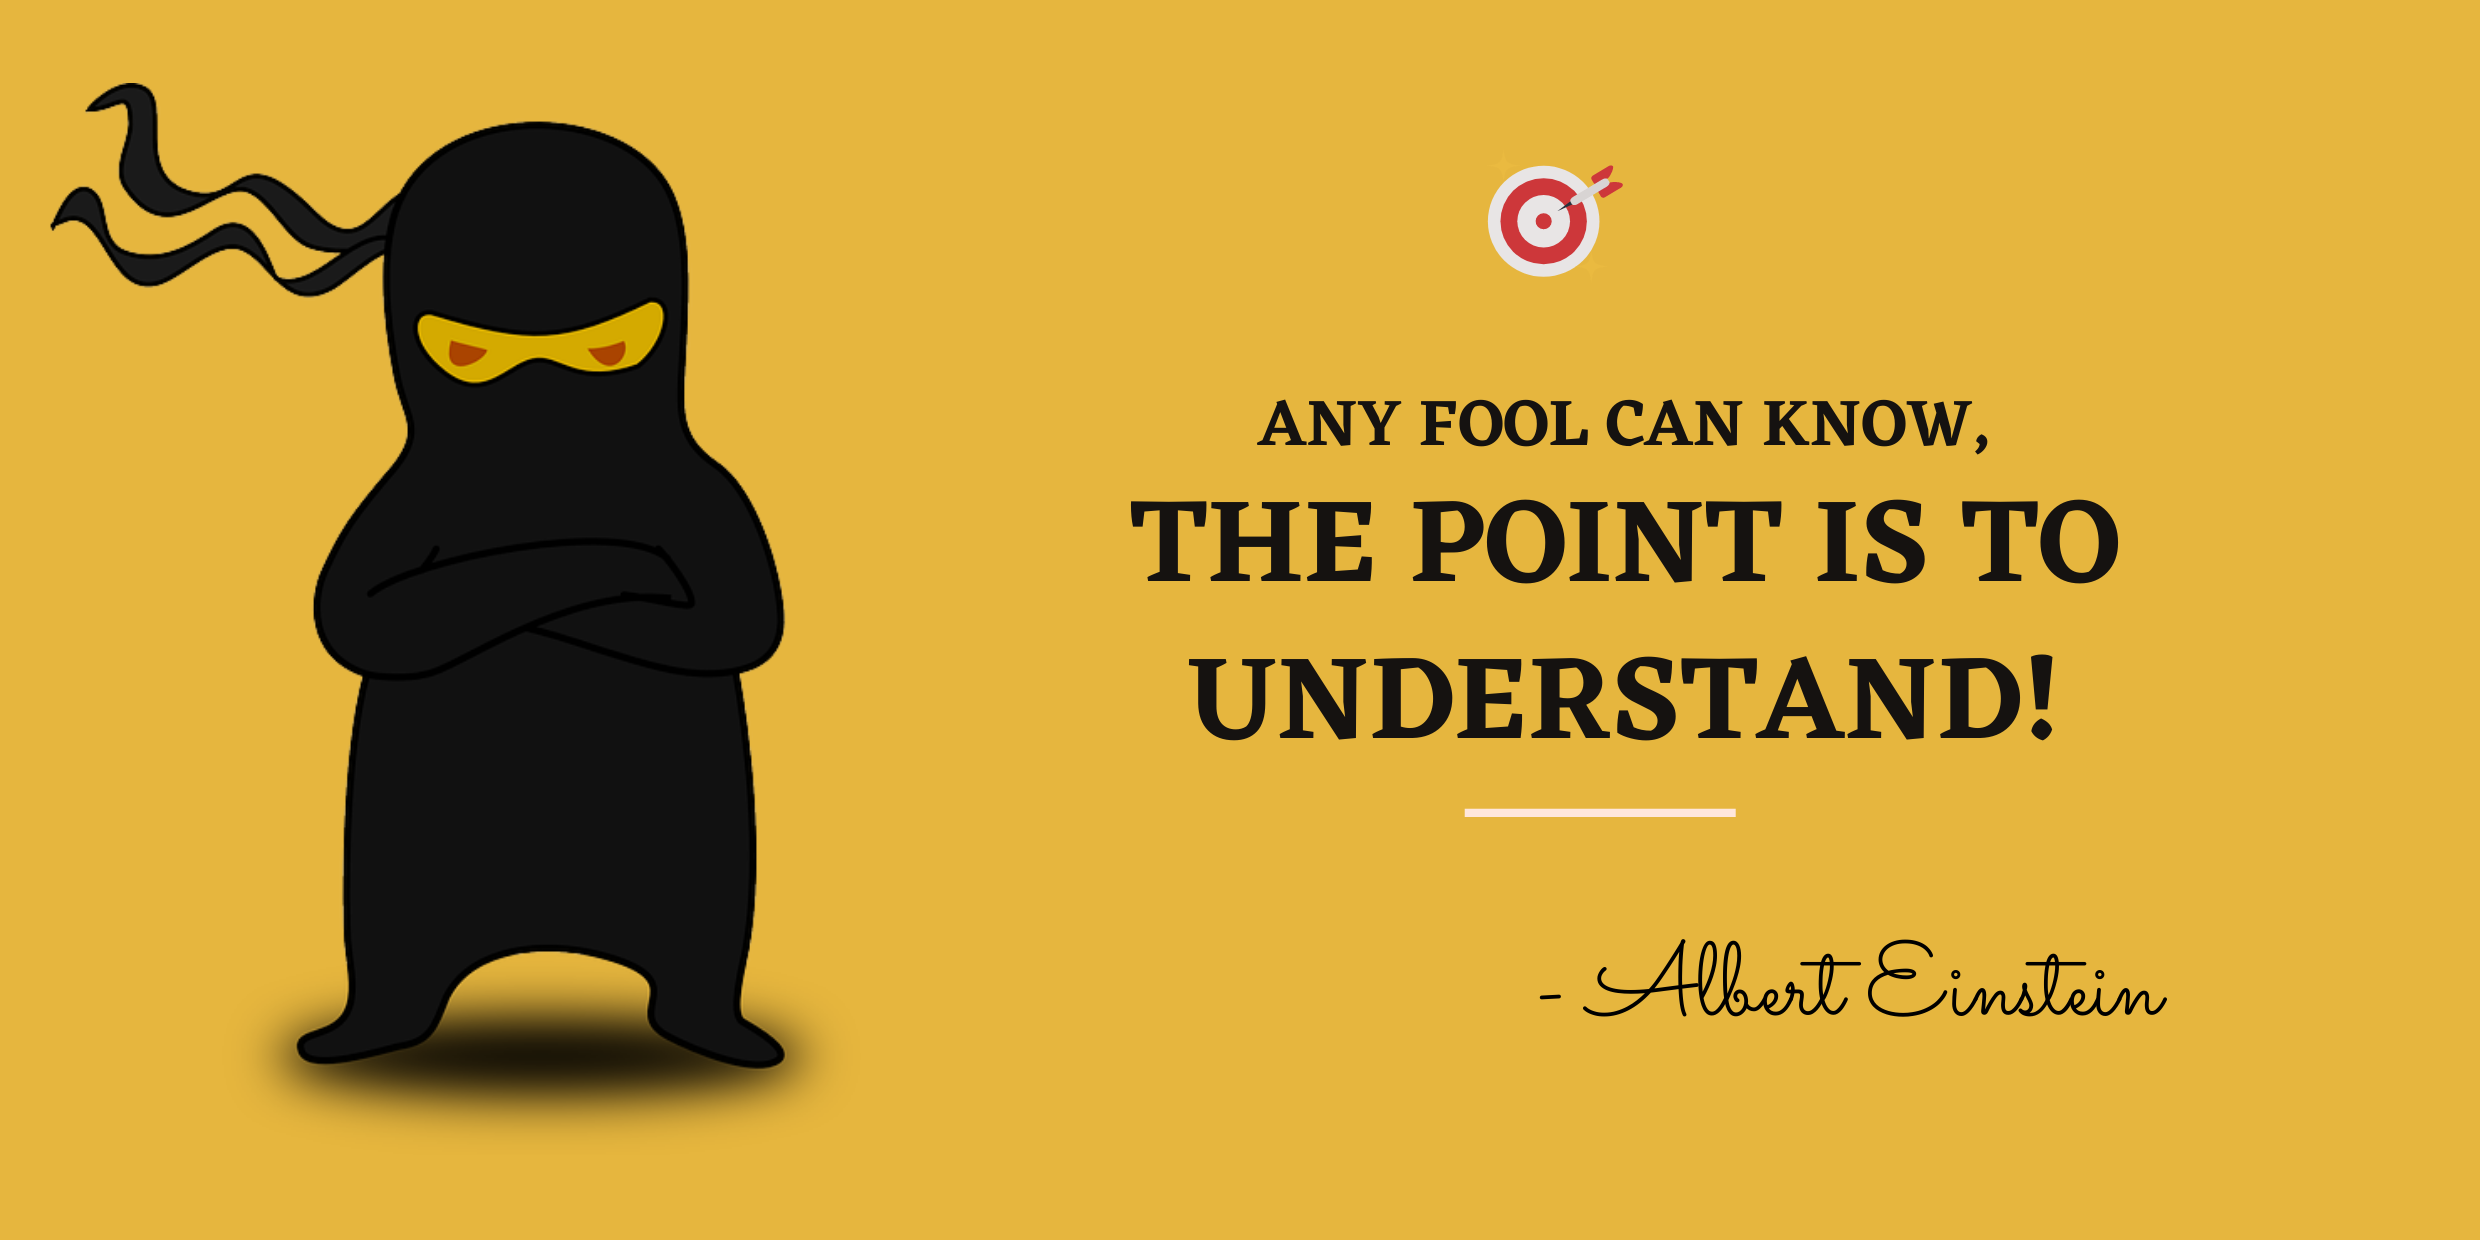
\includegraphics[scale=.2]{content/practise.jpg}
	\end{figure}	
	\begin{enumerate}
		\item \textbf{Which of the following command is used to search a file in a directory?}
		\begin{enumerate}[label=(\alph*)]
			\item grep
			\item sort
			\item cut
			\item find    %correct
 		\end{enumerate}
		\bigskip
		\bigskip	
		
		\item \textbf{Which of the following command is used to search an expression in a file?}
		\begin{enumerate}[label=(\alph*)]
			\item find
			\item locate
			\item grep   %correct
			\item sort          
		\end{enumerate}
		\bigskip
		\bigskip
		
		
		\item \textbf{Which of the following are valid options of find command? (Select all that applies.)}
		\begin{enumerate}[label=(\alph*)]
			\item -user            %correct
			\item -name            %correct
			\item -type           %correct
			\item -atime          %correct
		\end{enumerate}
		\bigskip
		\bigskip
		
		\item \textbf{Which of the following is valid options for grep command? (Select all that applies.)}
		\begin{enumerate}[label=(\alph*)]
			\item \textbf{-i}   %corrrect
  			\item \textbf{-r} or \textbf{-R}   %correct
			\item \textbf{-v}   %correct
			\item \textbf{-n}   %correct
		\end{enumerate}
		\bigskip
		\bigskip
		
		\item \textbf{Which of the following command is used to search all lines in \textbf{/etc/fstab} not having letter \textbf{"\#"}?}
		\begin{enumerate}[label=(\alph*)]
			\item grep -v "\#" /etc/pfstab  %correct
			\item grep -w "\#" /etc/pfstab  
			\item grep -n "\#" /etc/pfstab  
			\item grep -i "\#" /etc/pfstab  
		\end{enumerate}
		\bigskip
		\bigskip
		
		\item \textbf{Which of the following command is used to display first 20 lines of \textbf{/etc/passwd} file?}
		\begin{enumerate}[label=(\alph*)]
			\item head -2 /etc/passwd
			\item tail -20 /etc/passwd
			\item head -20 /etc/passwd   %correct
			\item tail -2 /etc/passwd
		\end{enumerate}
	
		\bigskip
		\bigskip
		\item \textbf{Which of the following command is used to sort all lines of \textbf{/etc/passwd} file in descending order?}
		\begin{enumerate}[label=(\alph*)]
			\item sort -d /etc/passwd
			\item sort -r /etc/passwd   %correct
			\item sort -n /etc/passwd
			\item sort -R /etc/passwd
		\end{enumerate}
	
		\bigskip
		\bigskip
		\newpage
		\item \textbf{Which of the following command is used to count number of words in a file?}
		\begin{enumerate}[label=(\alph*)]
			\item sort
			\item wc   %correct
			\item cut
			\item tail
		\end{enumerate}
	
		\bigskip
		\bigskip
		\item \textbf{Which of the following command is valid to display only UID of all users from \textbf{/etc/passwd} file?}
		\begin{enumerate}[label=(\alph*)]
			\item cut -d":" -f3 /etc/passwd  %correct
 			\item cut -d"." -f2 /etc/passwd
			\item cut -d":" -f1 /etc/passwd
			\item cut -d":" -f4 /etc/passwd
		\end{enumerate}
	\end{enumerate}
	
	
\end{flushleft}

\newpage

